%%%%%%%%%%%%%%%%%%%%%%%%%%%%%%%%%%%%%%%%%%%%
\subsubsection{Verify MCS performance [Daytime]}\label{secflow:prestudy}
In this sequence, we verify MCS performance to measure the fiber positions on focal plane.
We also check validity the PFS coordinate-transfer system.
Here, because MCS will arrive prior to PFI arrival\footnote{ASIAA also propose that MCS be aligned with the prime focus using pinhole array on POpt2 or FMOS/PIR, which is required after PFI arrival.}, there are two options for this test.
One is FMOS/PIR instead of fiber positioner system, and the other is pinhole array equipped to POpt2.

\paragraph{In the case of FMOS/PIR}
The field of view of FMOS ($\sim 30$ arcmin in diameter) is much smaller than that of PFS.
Besides, only 32 fibers can be back-illuminated simultaneously.
Nonetheless, the procedure of coordinate transformation shall be studied well.

MCS measures fiber positions somewhat converted to MCS frame, and then positions are transferred to them on focal plane.
On the other hand, FMOS fiber positioner (Echidna) measures fiber positions on the focal plane.
By comparing measured fiber positions by MCS and the coordinate transformation system, with those by Echidna, MCS function of measuring the fiber positions is verified.
%The error in measurement contributed by dome seeing temperature, or telescope elevation will be also estimated by measuring position several elevation and temperatures.
%% estimation of error is needed for PFI-MCS relation? maybe not. but error estimation is needed for measurement on MCS?
%% Echidna: 20 fibers are illuminated at a time
At present, Echidana can position fibers with the accuracy of $\sim 35$ um\footnote{Originally the fiber allocation was achieved with the accuracy of $\sim 10$um. Recently the encoder of X position of sky camera was broken, which have added $\sim 25$ um for fiber positions.}.
We set the goal in accuracy of fiber positioning 50 um for pre-study, the same as 1-st pass distortion map (\ref{secflow:1stDM}).

The procedure of the measurement is as follows:
\begin{enumerate}
\item Decide which fibers to move and which fibers not to move (like fixed fiducial fibers).
Figure \ref{fig:fibEchidna} shows an example.
%One way is to define  nine fixed fibers arranging 3 $\times$ 3 grid. 
\item Built distortion map of PIR from the MCS viewpoint (the form of $D_2$ for FMOS/PIR).
With all fibers back-illuminated, we take the fiber image at home position by MCS.
We also have the physical positions of FMOS fibers.
Using these positions, we will determine the form of the distortion map.
\item Define F3C for FMOS. 
In order to distinguish with F3C for PFS, we name the defined coordinate ``F3C(PIR)". 
``F3C(PIR)" is practically the same as the positions measured with the spine camera of Echidna.
With fixed fibers back-illuminated, we take fibers image by both MCS and Echidna, and then the positions of fixed fiducial fibers on F3C are measured.
\item Take all fibers image by MCS and calculate their position
\begin{enumerate}
\item Using image of fixed fibers, determine the transformation from MCS coordinate to F3C(PIR) coordinates, that is, the parameters of $D_2$ for FMOS/PIR). 
\item Using images of the rest fibers, calculate the positions on above coordinate frame.
\end{enumerate}
\item Measure fiber positions of FMOS/PIR, and compare with those derived on F3C(PIR)
\item Executing the above procedures for several fiber configurations at a various Elevation (EL) and Rotator angle (ROA), study the stability of the measurements.
\redtext{We may be able to study the effect of local surface error of corrector lens for coordinate transform by changing fiber configurations.} 
Here the error due to temperature and dome seeing is included.
We also examine these effect.
\end{enumerate}

%--------------------------------------------------------------
%  Figure: An example of fiber arrangement 
%--------------------------------------------------------------
\begin{figure}[!ht]
\begin{center}
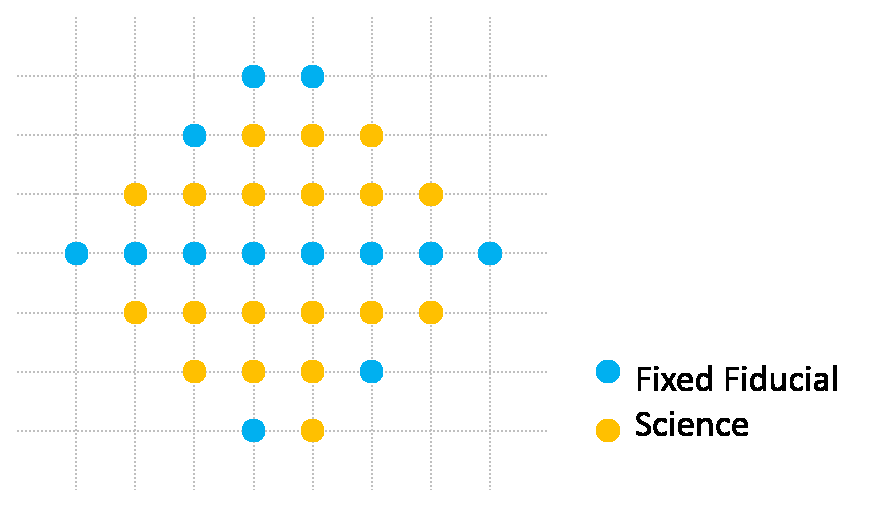
\includegraphics[width=100mm]{fiber_echidna.eps}
\end{center}
\caption{
Example of the arrangement of FMOS/Echidna back-lit fibers.
32 fibers can be back-illuminated at a time. }
\label{fig:fibEchidna}
\end{figure}

\paragraph{In the case of pinhole array on POpt2}
If pinhole array can be attached on the POpt2, we can study transfer coordinate system in the similar procedure above.
WFC has a ring-patterned local surface error with a pitch of 6mm, pinholes with the smaller pitch enable us to study the effect of the local surface error.
Using pinholes are arranged at fiducial fiber position and hexagonal position of 4 mm (half size of that of cobras), we will study the the coordinate transform in the following procedure.
\begin{enumerate}
\item Distortion map is determined with WFC as-built model.
\item \label{item:M4pin2} Take pin holes array images by MCS.
Choose one of the holes in the patrol areas and calculate their position on F3C.
\item Compare the calculated positions with the design.
\item Choosing the another holes, repeat \ref{item:M4pin2}.
\item Executing the above procedures at a various Elevation (EL) and Rotator angle (ROA), study the stability of the measurements.
\end{enumerate}

Because the corrector lens are different between PIR and WFC, we cannot study a effect of WFC itself if we use FMOS.
However, similar study will be performed by changing the fiber configurations (TBC).


\paragraph{Back-up plan}
If MCS would deliver at Subaru just before the arrival of PFI, we will not have enough time to practice the procedure of the coordinate transformation.
As back-up plan, we will use the camera which was used to measure dome seeing in 2012.

According to the report (http://sumire.pbworks.com/w/file/70195197/domeseeing3v1.pdf), the camera was equipped to the Caseggrain focus with NexStar4SE telescope.
In this configuration, the camera covers 100 mm $\times$ 120 mm of FMOS focal plane, which is large enough to illuminate 32 fibers, because neighboring fibers have 7mm separation.
The FWHM of the spot size on the camera will be 2.6 pixel, which is the same as that of the PFS fibers on MCS.

\begin{itembox}[l]{\suctitle{Success Criteria}}
MCS measures the fiber position consistent with that by Echidna at various telescope positions. 
The accuracy is less than 50 um.

\bluetext{Required long time to analyze the data?: Yes. \\
---It should take time to compare the positions derived with MCS with that by Echidna, and mature the coordinate transfer algorithm.
Once we obtained the data, we can use the same data to mature the algorithm.
}
\end{itembox}